\section{Six Sigma Approaches}
% Fundamentals and Handbook for process management
The first set of analysation and optimization techniques discussed in this chapter originate from the Six Sigma initiative. The name Six Sigma originates from the interval of $6\sigma$ in the normal distribution that indicates the aimed success rate of $99.99966\%$ \cite{siha2008business}\cite{vivekananthamoorthy2011lean} . A representation of the statistical meaning can be see in figure \ref{fig:six-sigma}. Apart from the goal to decrease the error rate, $6\sigma$ is also an methodology for systematically improving process quality \cite{tennant2017six}.

\begin{figure}[H]
		\centering
		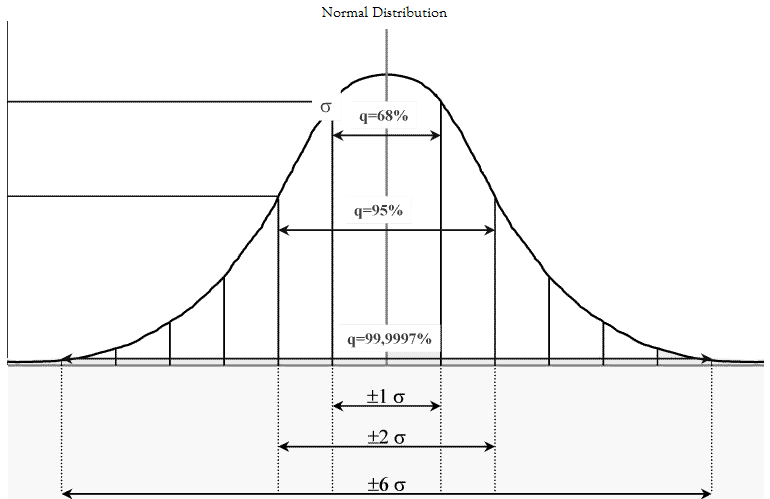
\includegraphics[width=0.9\columnwidth]{graphics/six-sigma}
		\caption{The standard normal distribution showing the $6\sigma$ interval (graphic from \cite{vivekananthamoorthy2011lean})} 
		\label{fig:six-sigma} 
\end{figure}



\subsection{Process Map}
\subsection{Check Sheets}
\subsection{Pareto Analysis}
\subsection{Cause and Effect Diagram}
\subsection{Root Cause Analysis}
\subsection{Quality Function Deployment (QFD)}

\section{Other Qualitative Measures}

\subsection{Value Added Analysis (VAA)}

\section{Quantitative Analysis}
% Fundamentals chapter 7
\subsection{Performance Measures}
\subsection{Flow Analysis}
\subsection{Queues}
\subsection{Simulation}

\section{Benchmarking Processes}

%H. Harrington - Business Process Improvement chapter 9 